\documentclass[final,5p,twocolumn]{elsarticle}
\usepackage{amsmath,amssymb,amsthm,booktabs,graphicx}
\usepackage[hidelinks]{hyperref}
\newtheorem{theorem}{Theorem}
\newtheorem{corollary}[theorem]{Corollary}
\newcommand{\dd}{\mathrm{d}}

\begin{document}
\begin{frontmatter}
\title{Decision invariance and boundary crossings in Gaussian prototype flows}
\begin{abstract}
Gaussian prototype scores define a classifier and a density-ascent flow that can
transport inputs before classification. For affine decision cells, we prove that
preservation of every strict decision at one positive horizon is equivalent to
preservation at all horizons. A finite criterion checks a weighted normal
balance of prototypes sharing a tangential projection onto each facet. For
equal-mass Voronoi sites, preservation at one variance at least a quarter of the
squared diameter forces a reflection-group orbit and implies preservation at
every variance. Generic multiclass configurations in dimension at least two
admit switches at every positive horizon. With shared anisotropy, Euclidean ascent also requires the
facet normals to be eigenvectors of the precision matrix. A local
whole-interval certificate uses the reachable tangential projection of a query.
On three public one-prototype cohorts, it can increase coverage relative to a
covariance-based certificate. We distinguish these exact-arithmetic guarantees
from numerical checks and from the effect of transport on class accuracy.
\end{abstract}
\begin{keyword}
Prototype classifiers \sep Gaussian mean shift \sep Decision boundary \sep
Flow invariance \sep Reflection group
\end{keyword}
\end{frontmatter}
\thispagestyle{plain}

\section{Introduction}

The classes of a Gaussian prototype classifier compete by their component
scores. The sum of those scores also supplies a vector field that can move an
input before the fixed readout is applied. Density ascent can change the
ordering of the class scores even though it increases the sum.
Classical mean shift and modal clustering concern the ascent to modes and
the basins of those modes \cite{carreira,chacon}. We ask when a prescribed
decision partition is preserved during transport. Power diagrams and
reflection-group orbit polytopes supply static geometric tools
\cite{aurenhammer,ardila}. Classical tangency criteria address invariance
under a vector field \cite{nagumo}. Here the premise is preservation under a
single sampled time map. We translate it into finite conditions on the
driving prototypes and use those conditions to derive practical
preservation tests.

\section{Exact invariance}

Let the driving prototypes be $a_i$ with positive masses $w_i$, common
variance $\beta>0$, and responsibilities
$\pi_i(x)\propto w_i e^{-\|x-a_i\|^2/(2\beta)}$ summing to one.
The vector field is $F(x)=\mu(x)-x$ with $\mu(x)=\sum_i\pi_i(x)a_i$.
It is the Euclidean gradient of
$U(x)=\beta\log\sum_i w_i e^{-\|x-a_i\|^2/(2\beta)}$.
The derivative
$DF=\operatorname{Cov}_{\pi}(a)/\beta-I$ is symmetric and bounded
since the prototypes are finite. Thus the flow $\Phi_t$ is complete
and depends analytically on the initial condition \cite{carrillo}.
The potential has compact superlevel sets.

Take a finite readout given by the maximum of distinct affine scores.
Ignore scores with no full-dimensional strict cell. With one distinct
Gaussian prototype per class, the shared quadratic term cancels to
give such a readout. Equal masses give the ordinary Voronoi diagram.
Let $H$ support a facet between full-dimensional cells, let $n$ be a
unit normal, and choose $o\in H$. Write $a_i=o+u_i+r_i n$ with
$u_i\perp n$. Define
\begin{equation}
 A_u=\sum_{i:u_i=u} w_i e^{-r_i^2/(2\beta)},\qquad
 B_u=\sum_{i:u_i=u} w_i r_i e^{-r_i^2/(2\beta)}.
 \label{eq:letter-balance}
\end{equation}

\begin{theorem}
\label{thm:letter}
Preservation of every strict decision cell at some fixed $T>0$ is
equivalent to preservation at every $t\ge0$ and to $B_u=0$ for
every tangential projection group on every facet plane.
\end{theorem}

\begin{proof}
If all strict cells are preserved at $T$, continuity maps the
relative interior of each common facet into both incident cell
closures. Analytic continuation of the normal coordinate of $\Phi_T$
along $H$ gives $\Phi_T(H)\subseteq H$. All iterates of a point in
$H$ at times $jT$ stay on $H$ and in a compact superlevel set.
Since $U$ increases to a limit along the sampled orbit, each
accumulation point $p\in H$ satisfies $U(\Phi_Tp)=U(p)$. The
difference is $\int_0^T\|F(\Phi_s p)\|^2\dd s$, hence $F(p)=0$.

The tangent space to $H$ is invariant under $D\Phi_T(p)=e^{TDF(p)}$.
The real symmetric $DF(p)$ has the same eigenspaces as its exponential.
It therefore splits into a tangential block $A$ and normal entry $b$.
If the restriction of the normal velocity to $H$ is nonzero, in
coordinates centered at $p$ it has a first nonzero homogeneous Taylor
term $Q_k(y)$ of degree $k\ge2$. A trajectory starting at $(y,0)$
has zero normal terms through degree $k-1$. Its normal term at
degree $k$ is
\[
 \int_0^T e^{b(T-s)}Q_k(e^{sA}y)\,\dd s .
\]
In a real eigenbasis of $A$, each monomial is multiplied by a
strictly positive real integral. This is the degree-by-degree operator
of flow embedding \cite{zhang,ribon}. It cannot send $Q_k$ to zero,
contradicting $\Phi_T(H)\subseteq H$. Thus the field is tangent on
$H$. This argument also covers zero eigenvalues.

On $H$ the normal velocity at $o+y$ is the ratio of
$\sum_u B_u e^{-\|y-u\|^2/(2\beta)}$ to
$\sum_u A_u e^{-\|y-u\|^2/(2\beta)}$. Factoring out the common
Gaussian leaves exponentials with distinct slopes. On a generic
line their successive derivatives form a Vandermonde system, so
they are independent. In dimension one there is a single group.
Therefore tangency implies all the
equalities in \eqref{eq:letter-balance}. Conversely they make the field
tangent on each supporting plane. Backward uniqueness prevents an orbit
from reaching such a plane from either open halfspace. A strict cell is
the intersection of its open facet halfspaces, proving preservation.
\end{proof}

With at least three equal-mass sites in dimension at least two,
almost every configuration has no third site on another pair's
bisector and no parallel differences between distinct pairs.
Each exposed facet then has a third site alone in its projection
group, with nonzero normal offset. Thus global preservation fails
at every positive horizon. Openness of the time map gives a set of
strict switched decisions of positive volume. This conclusion
concerns the existence of switches, with no lower bound on their
population mass.

\begin{corollary}
\label{cor:letter}
For one distinct equal-mass site per class, preservation at every
variance is equivalent to reflection symmetry in every Voronoi
facet, and to the sites being a single orbit of a finite orthogonal
reflection group in their affine span after translation. It follows
already from preservation at one positive horizon at
$\beta\ge D^2/4$ for site diameter $D$.
\end{corollary}

\begin{proof}
All equal-mass facets are independent of $\beta$. In
\eqref{eq:letter-balance}, independence of exponentials in $1/\beta$
requires cancellation of matching offsets $r$ and $-r$ when the
criterion holds for every $\beta$. Conversely reflection cancels
them. If $\beta\ge D^2/4$, the Hessian of $U$ is negative
semidefinite from the diameter bound on a one-dimensional
variance. The restriction to any line is analytic and tends to
$-\infty$ in both directions. It cannot have an affine segment,
so $U$ is strictly concave. Its unique stationary point attracts
every orbit: the orbit is bounded and $\|F\|^2$ tends to zero by
uniform continuity and its finite integral. If the cells are
invariant, that stationary point lies in every closed Voronoi cell.
The sites are cospherical about it and each facet plane contains it.
Projection groups on such a plane have at most two offsets, which
must be equal and opposite to balance.

The facet reflections generate a finite group, acting faithfully
on the sites in their affine span and fixing their centroid. The
action is transitive by connectedness of the Voronoi adjacency
graph, since each facet reflection exchanges its incident sites.
Conversely the Voronoi cells of a finite reflection orbit are
normal cones of the orbit polytope. Each cone is a union of
reflection chambers \cite{ardila}: a maximizer of a linear
functional from a chamber interior must lie in that closed chamber,
since reflection across a violated wall increases the functional.
The unique orbit representative in the closed chamber is consequently
the winner throughout its interior. Each exposed facet is supported
on a reflecting hyperplane.
\end{proof}

The proof uses the analytic gradient structure. For instance, a
rotation field can preserve every decision after a full revolution
while moving inputs across boundaries in between. For the
one-prototype model, the same balance criterion also characterizes
preservation by any single relaxed mean-shift update
$(1-\alpha)x+\alpha\mu(x)$, $0<\alpha\le1$. Necessity follows by
continuity from both cells. For sufficiency, the normal posterior
mean is strictly increasing in the normal position when the driving
sites have distinct normal projections. It agrees with the plane
on the plane itself. This holds for the two driving sites of a
Voronoi facet, and preserves the halfspaces under the update.

\section{Shared anisotropy}

For shared kernel precision $P/\beta$, with $P$ symmetric positive
definite, the Euclidean gradient field is $P(\mu-x)$. Its derivative
is $P\operatorname{Cov}_{\pi}(a)P/\beta-P$. The same sampled-time
argument applies because the potential still has compact superlevel
sets and the derivative is symmetric. On an invariant $H$,
$n^\top P x=n^\top P\mu(x)$ is bounded because $\mu$ stays in the
prototype hull. The left side is bounded on all of $H$ only if
$Pn=\lambda_n n$. Then the tangential and normal kernel factors
split, and the necessary and sufficient balance is
\[
 \sum_{i:u_i=u}w_i r_i e^{-\lambda_n r_i^2/(2\beta)}=0.
\]
The projected exponential slopes remain distinct because $P$
is invertible on the tangent space. With one site per class, plane
normals are proportional to $P(a_b-a_a)$. If $P$ is nonscalar,
almost every site pair has a difference outside all its eigenspaces.
This produces generic switches even for two classes. For example,
$P=\operatorname{diag}(2,1)$ and equal sites $\pm(1,1)$ have the
tie plane $2x_1+x_2=0$. At $(1,-2)$ the posterior mean is zero and
$P(\mu-x)=(-2,2)$ has a nonzero normal component. In contrast the
preconditioned flow $\mu-x$ preserves this plane and becomes the
spherical model under whitening \cite{carreira2000}.

\section{Finite-interval certificates}

For the spherical model, orient the plane normal toward the initial
query. On $H$ the normal velocity is a convex average of $B_u/A_u$.
Its outward component is bounded in magnitude by
$\epsilon=\max(0,-\min_u B_u/A_u)$.
Since $\partial_n(n^\top F)\ge-1$, a normal distance $s$ from $H$
satisfies $\dot s\ge -s-\epsilon$ until contact. Thus
$s_0>\epsilon(e^T-1)$ ensures strict preservation on this side.
Requiring the inequalities for all competing planes is conservative
and avoids a separate facet enumeration.

The whole-plane envelope can be tightened using the reachable
projection. The tangential drift is a convex average of the $u_i$
minus the tangential position. By variation of constants the
projection stays in
\[
 y_0+(1-e^{-T})\operatorname{conv}\big(
     \{0\}\cup\{u_i-y_0\}_i\big).
\]
The log of each weighted plane contribution $L_i$ relative to a reference site is
affine in $y$. Its extrema $\underline L_i,\overline L_i$ on the
projected tube are obtained from the listed generators.
Set $v_i=r_i+s_0/(e^T-1)$. Then
\[
 \sum_{i:v_i\ge0} v_i e^{\underline L_i}
 +\sum_{i:v_i<0} v_i e^{\overline L_i}>0
\]
suffices for preservation. It gives a uniform lower bound on the
shifted plane velocity numerator, so $\dot s>-s-s_0/(e^T-1)$
before any first contact and $s(T)>0$. For an equal-mass defining
pair the normal offsets cancel and their combined relative weight
is two. This test has an exact-arithmetic guarantee. It does not
include floating-point error enclosures.

\section{Numerical evidence}

\begin{figure*}[t]
\centering
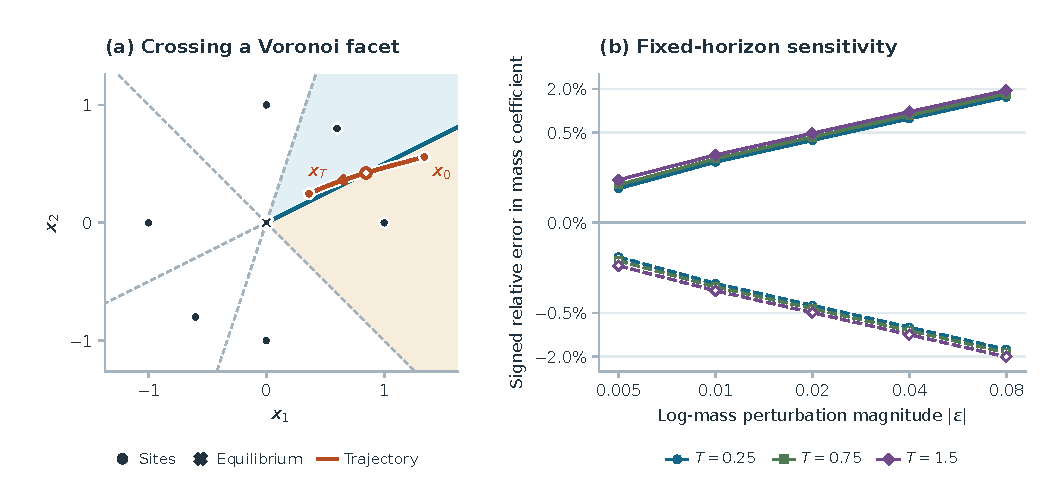
\includegraphics[width=0.86\textwidth]{figures/decision_invariance.pdf}
\caption{(a) Six equal-mass unit-circle sites share a stationary point.
The numerical trajectory crosses the highlighted Voronoi facet at
$t\approx0.748$ for $\beta=1.2$. (b) Relative error in the predicted
limit of the strip switch mass divided by $|\varepsilon|$, when a
single driving mass is perturbed and the affine readout stays fixed.
Solid lines and filled markers represent positive perturbations.
The ordinate uses a symmetric logarithmic scale.}
\label{fig:letter}
\end{figure*}

\paragraph{Controlled geometry}
The corners of a rectangle with equal masses satisfy the reflection
condition. A common attracting equilibrium is insufficient:
for the six sites $\{\pm(1,0),\pm(0,1),\pm(3/5,4/5)\}$ it occurs
at the origin when $\beta\ge1$, but the normal velocity on
$x=s(2,1)$, $s>0$, has a numerator proportional to
$e^{s/\beta}-e^{-s/\beta}$. A trajectory can cross that face
(Fig.~\ref{fig:letter}a). The supplementary study also gives a
weighted one-dimensional example of preservation without reflection
at a single variance.

\paragraph{Sensitivity at fixed time}
For the rectangle $(\pm1,\pm0.75)$ at $\beta=2$ with a fixed readout,
we perturb one log mass by $\varepsilon$. On the unperturbed
vertical facet the normal variation satisfies
$\dot\eta=\ell\eta+b$, with $\ell=-0.5$ and $b$ the weight derivative of
the normal field along the unperturbed path. The pulled-back boundary
shifts by $-\varepsilon\int_0^T e^{-\ell s}b(s)\dd s+o(\varepsilon)$.
We integrate the corresponding strip mass for a standard bivariate
Gaussian on the fixed window
$[-0.30,0.30]\times[0.30,1.20]$. A separate two-dimensional
integration locates the terminal-tie preimages. At horizons
$0.25$, $0.75$, and $1.50$, the limiting switch-mass coefficients
are $0.00875$, $0.02897$, and $0.06830$. Relative errors at
$|\varepsilon|=0.005$ are below $0.124\%$ for both perturbation
signs (Fig.~\ref{fig:letter}b). This is one controlled, unlabeled
example.

\paragraph{Interval comparison}
On the cospherical and rectangular fixtures, an outward-rounded
fixed-step integrator resolved all 51 terminal labels. It proved
29 whole-interval preservations and 10 departures, leaving 12
whole-path outcomes unresolved. The rectangle satisfies the
analytical reflection condition, so all its strict initial
decisions are invariant. The supplementary study gives the
validated step, fixed queries, and the separate endpoint and
whole-interval results.

\paragraph{External cohorts}
We fit one equal-mass centroid per class with training-only
standardization on Iris, Letter Recognition and UCI HAR
\cite{iris,letter,har}. The tests use 149 deduplicated Iris rows
in disjoint held-out folds, 3,620 Letter rows from the original
test set after screening for exact duplicates of training features,
and 864 windows from nine held-out HAR subjects. These cohorts
do not estimate variation across independent data sources.
At three horizons and two bandwidths we compare the plane
tests with a covariance-based whole-interval test. That test uses
a local bound on the posterior covariance to bound distances
and score variation along the trajectory. We compare endpoint
labels from DOP853 and refined RK4.

\begin{table*}[t]
\centering
\small
\setlength{\tabcolsep}{3.5pt}
\begin{tabular}{lrrrrrr}
\toprule
Source & Switch (\%) & $\Delta$ accuracy (pp) & ETD1 agrees (\%)
       & Whole-plane (\%) & Local plane (\%) & Covariance (\%)\\
\midrule
Iris & 2.68 & $+1.34$ & 100.00 & 49.66 & 96.64 & 93.29\\
Letter & 19.75 & $-1.38$ & 98.26 & 8.73 & 65.06 & 14.75\\
HAR & 6.37 & $-1.74$ & 99.77 & 32.29 & 86.23 & 30.32\\
\bottomrule
\end{tabular}
\caption{Endpoint switch rate, change in ordinary accuracy, one-step
exponential Euler (ETD1) agreement with the numerical endpoint, and
preservation certificate coverage at $\sqrt{\beta}/D=0.35$ and $T=0.50$.}
\label{tab:letter}
\end{table*}

At $T=0.50$ the local test certified 65.06\% of Letter and
86.23\% of HAR queries for the smaller bandwidth (Table~\ref{tab:letter}).
At $T=1.25$ the two comparison certificates abstained on every
query from those two datasets. At the larger bandwidth, the local
test still covered 13.37\% and 44.79\%, respectively.
No accepted query left its decision region at the sampled
checkpoints in any of the 18 source--horizon--bandwidth
combinations. DOP853 and refined RK4 agreed on the endpoint labels.
The checks concern the stated cohorts and exact-arithmetic
conditions evaluated numerically. On the first held-out fold of
each source at the Table~\ref{tab:letter} setting, the local guard
with RK4 fallback took 1.04, 2.03, and 0.34 times the full-RK4
latency on Iris, Letter, and HAR, respectively, with the same
endpoint labels. The timing excludes one-time setup. A synthetic
scaling check measured a slowdown at 40 classes despite high
coverage. These costs depend on the number of rival sites,
geometry, hardware, and batch size.

\section{Discussion}

The theorem precludes recovering all initial decisions at a
special positive sampling time when the flow is transverse to any
active affine face. The reachable-projection bound can still certify
many individual inputs, with coverage that varies by geometry and
horizon. Classification harm depends on which decisions change
and the true class law there. A separate locked core-only study
with multiple fitted prototypes per class illustrates this distinction.
At the primary setting, one ETD1 step predicted endpoint changes
about as well as a projected-margin score on the same queries,
and the selective covariance solver reduced field evaluations while
increasing latency. The supplementary study details those controls,
a tangency extension for connected regular curved interfaces, and
the limitations of the numerical validations.

\paragraph{Data, code, and research workflow}
The supplementary study documents data digests, commands, and
results. OpenAI Codex assisted in developing candidate proofs,
implementing analysis drivers and plotting code, and conducting
independent agent checks. The reported numbers are outputs of the
documented deterministic analyses and numerical solvers.

\section*{Generative AI and manuscript preparation}
OpenAI Codex was used to review literature, help structure and edit
the manuscript, and prepare drafts. This version is provided for
author review.

\begin{thebibliography}{13}
\bibitem{carreira} M. A. Carreira-Perpi\~n\'an, Gaussian mean-shift is an EM algorithm, IEEE TPAMI 29 (2007) 767--776. \href{https://doi.org/10.1109/TPAMI.2007.1057}{DOI}.
\bibitem{chacon} J. E. Chac\'on, A population background for nonparametric density-based clustering, Stat. Sci. 30 (2015) 518--532. \href{https://doi.org/10.1214/15-STS526}{DOI}.
\bibitem{aurenhammer} F. Aurenhammer, Power diagrams: Properties, algorithms and applications, SIAM J. Comput. 16 (1987) 78--96. \href{https://doi.org/10.1137/0216006}{DOI}.
\bibitem{ardila} F. Ardila, F. Castillo, C. Eur, A. Postnikov, Coxeter submodular functions and deformations of Coxeter permutahedra, Adv. Math. 365 (2020) 107039. \href{https://doi.org/10.1016/j.aim.2020.107039}{DOI}.
\bibitem{nagumo} M. Nagumo, \"Uber die Lage der Integralkurven gew\"ohnlicher Differentialgleichungen, Proc. Phys.-Math. Soc. Japan 24 (1942) 551--559. \href{https://doi.org/10.11429/ppmsj1919.24.0_551}{DOI}.
\bibitem{carrillo} S. A. Carrillo, A quick proof of the regularity of the flow of analytic vector fields, C. R. Math. 359 (2021) 1155--1159. \href{https://doi.org/10.5802/crmath.271}{DOI}.
\bibitem{zhang} X. Zhang, The embedding flows of $C^\infty$ hyperbolic diffeomorphisms, J. Differ. Equ. 250 (2011) 2283--2298. \href{https://doi.org/10.1016/j.jde.2010.12.022}{DOI}.
\bibitem{ribon} J. Rib\'on, Embedding smooth and formal diffeomorphisms through the Jordan--Chevalley decomposition, J. Differ. Equ. 253 (2012) 3211--3231. \href{https://doi.org/10.1016/j.jde.2012.09.009}{DOI}.
\bibitem{carreira2000} M. A. Carreira-Perpi\~n\'an, Mode-finding for mixtures of Gaussian distributions, IEEE TPAMI 22 (2000) 1318--1323. \href{https://doi.org/10.1109/34.888716}{DOI}.
\bibitem{iris} R. A. Fisher, Iris, UCI Machine Learning Repository (1936). \href{https://doi.org/10.24432/C56C76}{DOI}.
\bibitem{letter} D. J. Slate, Letter Recognition, UCI Machine Learning Repository (1991). \href{https://doi.org/10.24432/C5ZP40}{DOI}.
\bibitem{har} J. L. Reyes-Ortiz, D. Anguita, A. Ghio, L. Oneto, X. Parra, Human Activity Recognition Using Smartphones, UCI Machine Learning Repository (2013). \href{https://doi.org/10.24432/C54S4K}{DOI}.
\end{thebibliography}
\end{document}
